% Created 2019-07-11 Thu 12:21
% Intended LaTeX compiler: pdflatex
\documentclass[11pt]{article}
\usepackage[utf8]{inputenc}
\usepackage[T1]{fontenc}
\usepackage{graphicx}
\usepackage{grffile}
\usepackage{longtable}
\usepackage{wrapfig}
\usepackage{rotating}
\usepackage[normalem]{ulem}
\usepackage{amsmath}
\usepackage{textcomp}
\usepackage{amssymb}
\usepackage{capt-of}
\usepackage{hyperref}
\usepackage{listings}
\usepackage[left=1in,top=1in,right=1in,bottom=1in]{geometry}
\usepackage{palatino}
\usepackage{fancyhdr}
\usepackage{sectsty}
\usepackage{engord}
\usepackage{cite}
\usepackage{graphicx}
\usepackage{setspace}
\usepackage[compact]{titlesec}
\usepackage[center]{caption}
\usepackage{multirow}
\usepackage{ifthen}
\usepackage{longtable}
\usepackage{color}
\usepackage{amsmath}
\usepackage{listings}
\usepackage{pdfpages}
\usepackage{nomencl}	% For glossary
\usepackage{pdflscape}	% For landscape pictures and environment
\usepackage{verbatim} 	% For multiline comment environments
\usepackage[table]{xcolor}
\author{eo shiru}
\date{\today}
\title{SVS - Lectures}
\hypersetup{
 pdfauthor={eo shiru},
 pdftitle={SVS - Lectures},
 pdfkeywords={},
 pdfsubject={},
 pdfcreator={Emacs 26.2 (Org mode 9.1.9)}, 
 pdflang={English}}
\begin{document}

\maketitle
\tableofcontents

Distributed Solution Design\\
\begin{center}
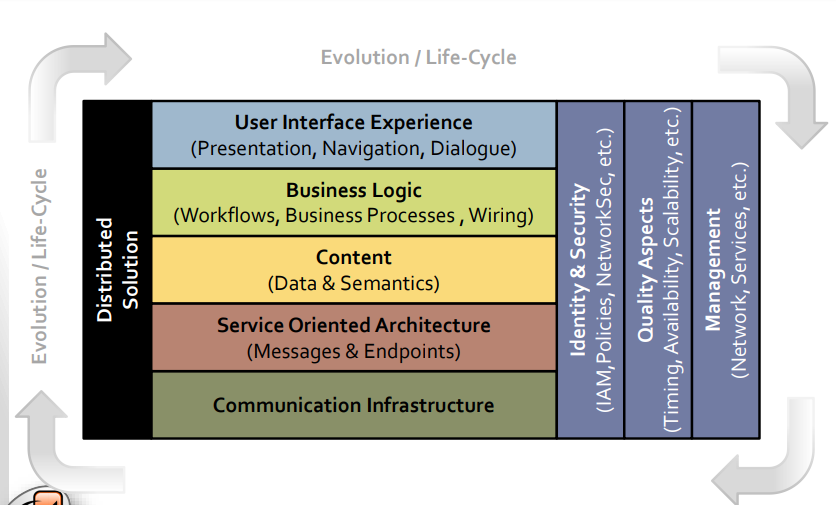
\includegraphics[width=.9\linewidth]{/home/eoshiru/library/docs/knowledge-database/static/images/distributed-solution-design.png}
\end{center}

The increasing decentralization of public networks by deregulation of telecommunications markets leads to increasingly extensive use of the Web and increasing usage of the open \& decentralized Internet. Back then networks were mostly closed and managed centrally, while the Internet was used as a pure research and didn't have worthwile targets. Because of the recent evolution of the internet and the world wide web security mechanisms are becoming an indispensable part of modern communication systems. Security must be considered in a comprehensive \& integrated way, taking new aspect into account: identity and privacy.\\
But what is \textbf{security}? Security refers to the ability to avoid being harmed by any risk, danger or threat (Cambridge Dictionary of English). In practice and regarding IT infrastructure this is an \emph{unreachable goal}. Therefore your software is never a 100\% secure.

\subsubsection{Security Goals}
\label{sec:orge3676b6}
Our focus is on actions to achieve security goals.\\
Mnemonic for security goals: "\textbf{CIA}":
\begin{itemize}
\item Confidentiality
\begin{itemize}
\item data secrecy
\end{itemize}
\item Integrity
\begin{itemize}
\item data intactness
\end{itemize}
\item Authenticity
\begin{itemize}
\item secure data origin
\end{itemize}
\item additional (soon-to-be) major goals:
\begin{itemize}
\item Liability (Non-Repudiability)
\begin{itemize}
\item non-repudiation (repudiation = Zurückweisung, Nichtanerkennung) of data origin
\item important for contracts or in the fight against SPAM
\end{itemize}
\item Identity
\begin{itemize}
\item verification of an individual entity
\item nowadays identity is of increasing significance
\end{itemize}
\end{itemize}
\end{itemize}

In this lecture the generic term \textbf{Assets} denotes things worth protecting eg data or services (business applications for example).

A strong physical security is the foundation to protecting assets and achieving the security goals. Physical vs Digital Security:\\
\begin{center}
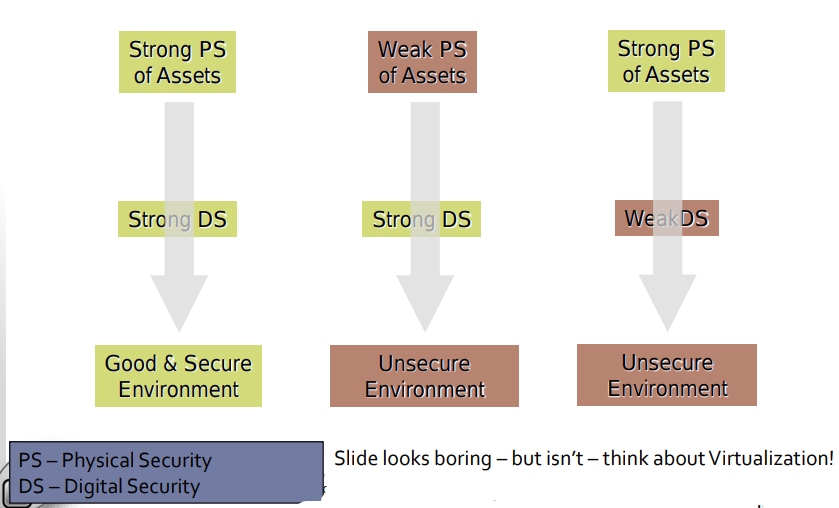
\includegraphics[width=.9\linewidth]{/home/eoshiru/library/docs/knowledge-database/static/images/physical-digital-security.png}
\end{center}
We can achieve the security goals mentioned in the previours lecture by:
\begin{itemize}
\item information encryption
\item implementation of authentication
\item establishment of security activities
\item monitoring of the system or the network in terms of attacks
\item continous reduction of weak spots
\item etc
\end{itemize}

\begin{center}
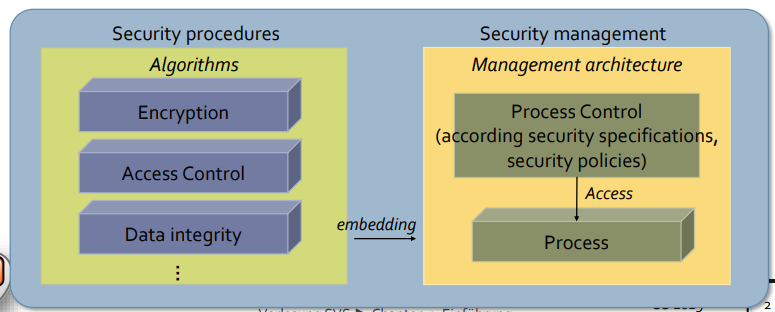
\includegraphics[width=.9\linewidth]{/home/eoshiru/library/docs/knowledge-database/static/images/security-procedures.png}
\end{center}

In the data transfer model (2 users communicating) we can distinguish for example two types of attackers:
\begin{itemize}
\item passive attacker
\begin{itemize}
\item can only listen, not manipulate
\item confidentiality threat
\end{itemize}
\item active attacker
\begin{itemize}
\item can listen, change, delete, duplicate
\item threat for confidentiality, integrity and authenticity
\end{itemize}
\end{itemize}

The difference between authenticity and liability lays in the focus between internal and external relationships. Here's an example: Authenticity means that Bob is sure the data comes from Alice (internal) - Liability means that Bob can prove this to third parties (external).

Here are some types of threats:
Interception of transmitted data
\begin{itemize}
\item Modification of transmitted data
\begin{itemize}
\item Change
\item Delete
\item Insert
\item Reorder data blocks
\end{itemize}
\item Masquerade
\begin{itemize}
\item Faking a false identity
\item Sending messages with a false source address
\end{itemize}
\item Unauthorized access to systems
\begin{itemize}
\item Keyword „Hacking”
\end{itemize}
\item Sabotage (Denial of Service)
\begin{itemize}
\item Causing an overload situation (including hardware)
\item “Destroying” protocol instances by illegal packets
\end{itemize}
\end{itemize}

And here are \emph{some} attack techniques:
Tapping cables or radio links
\begin{itemize}
\item Interposing (man-in-the-middle attack)
\item Replaying of intercepted messages (replay attack) (e.g. replay of login messages for the purpose of unauthorized access)
\item Selective changing / swapping of bits or bit strings (without being able to decrypt the message)
\item Break-in by taking advantage of errors (buffer overflows)
\item Break-in by means of active components (trojans, worms, backdoors)
\item Breaking cryptographic algorithms
\item Social Engineering (e.g. through direct contact and social web)
\end{itemize}

And some countermeasures:
\begin{itemize}
\item Don‘t use self-made algorithms, use only proven algorithms that are considered safe!
\item Use safe methods and replace old algorithms
\item Behaviour (Pattern) analysis
\item Use Social Web the right way
\item Know your enemy
\item limit the attack surface
\item limit identity properties
\item distribute attack surface
\item apply encryption everywhere
\end{itemize}

Security should be considered in an integrated way. This means:
\begin{itemize}
\item consideration of all assets
\item based on risk assesment
\item use adequate security approaches and services (often a mix of different techniques)
\end{itemize}

All in all it is almost impossible to achieve 100\% security. Therefore one has to clearly define what has to be protected and how high the according security requirements should be.

\subsection{Excourse: GDPR}
\label{sec:org840614e}
\textbf{What is a data subject?}
\begin{itemize}
\item any person whose personal data is being collected, held or processed
\end{itemize}

\textbf{What are the data subject's rights?}
\begin{itemize}
\item Individuals/Citizen (data subjects) have the right to:
\begin{itemize}
\item information about the processing of your personal data
\item obtain access to the personal data held about you
\item ask for incorrect, inaccurate or incomplete personal data to be corrected
\item request that personal data be erased when it’s no longer needed or if processing it is unlawful
\item object to the processing of your personal data for marketing purposes or on grounds relating to your particular situation
\item request the restriction of the processing of your personal data in specific cases
\item receive your personal data in a machine-readable format and send it to another controller (‘data portability’)
\item request that decisions based on automated processing concerning you or significantly affecting you and based on your personal data are made by natural persons, not only by computers; You also have the right in this case to express your point of view and to contest the decision
\end{itemize}
\end{itemize}

\textbf{What is personal data and what not?}\\
\(\rightarrow\) Personal data is any information that relates to an identified or identifiable living individual. Different pieces of information, which collected together can lead to the identification of a particular person, also constitute personal data.\\
Personal data that has been de-identified, encrypted or pseudonymised but can be used to re-identify a person remains personal data and falls within the scope of the law.\\
Personal data that has been rendered anonymous in such a way that the individual is not or no longer identifiable is no longer considered personal data. For data to be truly anonymised, the anonymisation must be irreversible.\\
Examples of personal data:
\begin{itemize}
\item name and surname, home adress, email adress
\item identification card number
\item location data
\item IP adress
\item cookie ID
\end{itemize}

Examples of data not considered personal data:
\begin{itemize}
\item a company registration number
\item an email adress such as info@company.com
\item anonymised data
\end{itemize}

\textbf{What is a data controller?}\\
The controller or data controller is simply the organization (a legal person, agency, public authority, etc.) or the natural person which, alone or depending on the organization and personal data processing activity, in collaboration with others defines what needs to happen with the personal data (and also collects personal data) and obviously is key in personal data protection.
Formal definition (Article 4):\\
\emph{‘controller’ means the natural or legal person, public authority, agency or other body which, alone or jointly with others, determines the purposes and means of the processing of personal data; where the purposes and means of such processing are determined by Union or Member State law, the controller or the specific criteria for its nomination may be provided for by Union or Member State law}



\textbf{What is a data processor?}\\
The processor or data processor is a person or organization who deals with personal data as instructed by a controller for specific purposes and services offered to the controller that involve personal data processing (remembering that processing can be really many things under the GDPR). The formal definition of the processor as you can read it in the GDPR Articles (GDPR Article 4):\\
\emph{Processor means a natural or legal person, public authority, agency or other body which processes personal data on behalf of the controller.} The main difference to data controllers is that the GDPR has a really different stance with regards to data processors whereby they have duties and responsibilities that are directly applicable and can be directly enforced and GDPR compliance is a shared obligation as you will discover.
\section{Attacks on End Systems}
\label{sec:orgd720a9b}
Attacks on end systems via
\begin{itemize}
\item computer viruses
\item computer worms
\item trojan horses
\item exploits
\item cracking systems
\end{itemize}

might focus on
\begin{itemize}
\item unsecured computer systems
\item exploiting programming errors
\item bad security measures
\item weak passwords
\end{itemize}


Computer Virus
\begin{itemize}
\item based on biological model
\item infects resources of the host system to replicate itself
\item malicious functions
\begin{itemize}
\item load generation
\item data corruption
\item spying
\end{itemize}
\item various types
\begin{itemize}
\item boot sector viruses
\item file viruses
\item macro viruses
\item script viruses
\item composites
\end{itemize}
\item self-defense mechanisms of viruses:
\begin{itemize}
\item stealth
\item modification
\item cryptographic methods
\item polymorphism
\item retroviruses (against anti-virus programs)
\end{itemize}
\item passive distribution: by embedding into other programs and execution by the host system
\end{itemize}

Computer Worm
\begin{itemize}
\item based on biological model
\item uses resources of the host system and of the network to spread over to other systems \emph{automatically} in order to execute its malicious function there
\item malicious functions
\begin{itemize}
\item load generation
\item data corruption
\item spying
\item spamming
\item DDoS
\end{itemize}
\item various types
\begin{itemize}
\item email worms (social worms, file attachment, active content)
\item interactive worms (ask the user "please press OK" to use exploits)
\item instant messaging worm (sending of malicious software / links to all chat partners)
\item IRC worms (usage of scripting in IRC programs)
\item P2P worms (at file-sharing sites: tempting names \(\rightarrow\) download)
\item cell phone worms (distribution via Bluetooth, MMS, etc)
\end{itemize}
\item often in combination with other forms of malware, eg viruses droppers, backdoors, trojans
\end{itemize}

Dropper (virus dropper, DDoS dropper)
\begin{itemize}
\item executable program that acts as a carrier program for malware
\item is usually terminated after the virurs has been installed
\end{itemize}

Injector
\begin{itemize}
\item similar to dropper, but the malware will only be "installed" (injected) in memory
\end{itemize}

Backdoor
\begin{itemize}
\item part of a program that allows users to gain acces to the machine / system bypassing the normal access security
\item variants: default passwords (BIOS); specially equipped passwords / routines / servers that allow access (sometimes subsequently installed programs)
\item closely linked to trojans and droppers
\end{itemize}

Trojan (trojan horse)
\begin{itemize}
\item similar to the well-known story..
\item program that executes a potentially harmful function without user's knowledge
\item attention: often mixed up in the context of rootkits and backdoors
\end{itemize}

Rootkit (administrator toolbox)
\begin{itemize}
\item collection of software tools for concealment and stealth intrusions of malicious software
\item examples: hiding backdoors by hiding processes, logs, log-ins
\end{itemize}

Exploit
\begin{itemize}
\item a program (including scripts \& macros) that exploits the weaknesses or failures of a system or another application to obtain privileges or to use it for DoS attacks
\end{itemize}

\textbf{Malware} as generic term refers to malicious or unwanted software or programs.

Buffer Overflow
\begin{itemize}
\item application reserves a buffer to store some input values
\item the length of the input is larger than the buffer but the whole input still gets processed
\item memory space outside the buffer gets overwritten/accessed
\end{itemize}

\section{Attacks on Infrastructures}
\label{sec:orgbcdbff9}
Attacks on infrastructures via
\begin{itemize}
\item attacks on signaling mechanisms
\item distributed denial of service (DDoS)
\item attacks on WLAN hotspots and routers
\item break-ins (password theft, bugs, exploits)
\end{itemize}

might focus on
\begin{itemize}
\item unsecured intermediate system
\item overload situations
\item unsecure data storage
\item weak passwords
\end{itemize}

Attacks on signaling mechanisms
\begin{itemize}
\item ICMP: fake control messages
\item RSVP: fake resource allocation
\end{itemize}

Attacks on router
\begin{itemize}
\item attacks on routing protocols
\item distribution of false routes
\item WLAN, Bluetooth etc
\end{itemize}

Attacks on Hardware, eg virtual server
\begin{itemize}
\item usb-attacks
\end{itemize}

Denial of Service Attack
\begin{itemize}
\item the targeted weak spot is the overload of the network component
\begin{itemize}
\item may result in loss of service or entire computer systems
\end{itemize}
\item attack possibilities
\begin{itemize}
\item basic principle: large amount of requests sent to the target service or target system
\item requests must be designed in a way that they lead to an overload situation (more efficient use of exploits)
\end{itemize}
\item examples:
\begin{itemize}
\item ping of death = fake "echo request" information leads to a crash
\item smurf = broadcasting of an ICMP "echo request" with false return address (address of the victim)
\end{itemize}
\item special forms
\begin{itemize}
\item \textbf{Distributed} DoS = coordinated attack with a large number of computers
\begin{itemize}
\item closely linked with trojan / droppers infected systems that can be used as a remote-controlled attack network (BotNets)
\item BotNets - Malware starts its DDoS attacks after being distributed via a dropper
\end{itemize}
\end{itemize}
\end{itemize}

WLAN Attacks
\begin{itemize}
\item the targeted weakspot is the transmission medium as well as utilizing encryption techniques
\item attack scenario
\begin{itemize}
\item capture data packets of a protected WIFI network
\item "attack" on encryption \(\rightarrow\) search for a key
\item use the found key for further attacks in the protected network
\end{itemize}
\item examples: wepcrack, weplab etc.
\end{itemize}

Break-in
\begin{itemize}
\item the targeted weakspots are routers, proxys, computers and services in a network as well as weak passwords, poor and faulty security mechanisms
\item attack scenarios
\begin{enumerate}
\item \emph{host scanning} \(\rightarrow\) which computer / router / proxy exist in close proximity of the target (broadcasts, routing list, traffic, sniffing, DNSpredict/Google)? \(\rightarrow\) list of target systems
\item \emph{scanning the target system} \(\rightarrow\) type of systems (by means of fingerprints, traffic analysis, Google, whois, etc.)  which services (IP/TCP/UDP) are available or vulnerable (portscanning \& ICMP etc)
\item \emph{attack} \(\rightarrow\) exploiting bugs, backdoors, exploits, password scanners/lists, dropper, GoogleHackingDB
\item \emph{successfull breach} \(\rightarrow\) read password lists, install droppers, backdoors, keyloggers, proxy monitor, rootkit, etc
\begin{itemize}
\item start attacks from the compromised system
\item remove traces
\end{itemize}
\end{enumerate}
\item examples:
\begin{itemize}
\item GHDB \(\rightarrow\) default SSID and passwords of WIFI routers
\item NBTEnum \(\rightarrow\) search for other Windows systems
\item Network Monitors \(\rightarrow\) traffic analysis (eg TTL field observations) with respect to transparent bridges or dangers arising from IDS (not to attract attention)
\end{itemize}
\item break-in via exploits for example toolkits, known exploits, zero day exploits
\end{itemize}

\section{Attacks on Data / Protocols}
\label{sec:org4725bbb}
Attacks on data / protocols via
\begin{itemize}
\item communication interception
\item information manipulation
\item attacks on protocols and core mechanism
\end{itemize}

Focus on
\begin{itemize}
\item protocol weaknesses
\item (lack of) communication weaknesses
\item focus on manipulating algorithms and protocols (eg via "contributions" to open source projects)
\end{itemize}

Examples:\\
\subsubsection{Address Resolution Protocol}
\label{sec:org2a709a9}
\begin{itemize}
\item \textbf{weak spot} of the ARP is that it is a stateless protocol and therefore it is possible to send ARP-Replies without any requests
\item \textbf{ARP-Spoofing} (ARP Request Poisoning, ARP Poison Routing)
\begin{itemize}
\item sniffing = collecting network information
\item poisoning = targeted sending of wrong ARP packets (ARP-Reply with MAC adress for a foreign IP adress) to caches
\item data packets will now be sent to attacker (address in the cache) which manipulates/spies on the data packets before they are sent to their real destination \(\rightarrow\) this faked association enables Man-in-the-Middle attacks
\end{itemize}
\item there are various tools to simplify attacks eg \href{https://www.youtube.com/watch?v=RTXAUJ2yqCg}{ARP Video}
\end{itemize}

\subsubsection{Internet Protocol}
\label{sec:org4a2f016}
\begin{itemize}
\item \textbf{weak spot} of the IP is that IP-packets are not protected
\item \textbf{attack possibilities}
\begin{itemize}
\item reading IP-packets is simple
\item checksums for integrity checking are not safe
\item no protection of IP-PCI (IP Header) \(\rightarrow\) manipulation of the protocol header is simple
\item liability is unsafe because authenticity of addresses is not provable
\end{itemize}
\item \textbf{attack scenario}
\begin{itemize}
\item target system is protected by IP-sender adresses (meaning that only systems with registered IP addresses are alllowed to use the target system)
\item sniffing: spying of systems that exchange data with the target system (can also be encrypted)
\item connecting to the target system using spied out IP addresses
\end{itemize}
\end{itemize}

\subsubsection{Transmission Control Protocol (TCP)}
\label{sec:org7b1905a}
\begin{itemize}
\item \textbf{weak spot} of TCP is that a large number of ACK messages leads to high load on the firewall control
\begin{itemize}
\item ACK = acknowledgement; TCP is an acknowledgement-based protocol; when computers communicate via TCP, received packets are acknowledged by sending back a packet with ACK bit set
\item some firewalls check incoming home network internet traffic insufficiently
\item verification only for SYN messages, ACK messages are all let through
\begin{itemize}
\item SYN =  synchronize message via which a client requests a connection from the server
\item part of the TCP three-way handshake (SYN \(\rightarrow\) SYN-ACK \(\rightarrow\) ACK)
\end{itemize}
\end{itemize}
\item \textbf{attack possibilities}
\begin{itemize}
\item incorrect ACKS are used to implement exploits (rather unproblematic)
\item ACK-Tunneling = ACK is used for data transport \(\rightarrow\) Trojan/Dropper acts as an ACK server and reads fata from the ACK (problematic)
\item \href{https://en.wikipedia.org/wiki/SYN\_flood}{SYN flood}
\end{itemize}
\item \textbf{attack scenario}
\begin{itemize}
\item intrusion into the target system and installation of an ACK server, which acts as a remote shell, or dropper, etc
\item target system can now be controlled remotely (until replacement by a better firewall)
\end{itemize}
\end{itemize}

\subsection{Web-based attacks}
\label{sec:org67b6336}
\subsubsection{SQL Injection}
\label{sec:orgee8e62e}
\begin{itemize}
\item \textbf{weak spot}: web applications that use databases and without properly sanatizing etc
\item \textbf{attack possibilities}
\begin{itemize}
\item transfer of input data to the database (Form, URL) in a way to spy, change, delete data and execute code
\end{itemize}
\end{itemize}
\subsubsection{XSS - Cross Site Scripting}
\label{sec:org5943793}
\begin{itemize}
\item \textbf{weak spot}
\begin{itemize}
\item possibility of executing script code in the browser
\item weak user input checks
\end{itemize}
\item \textbf{attack possibilities}
\begin{itemize}
\item identify weak spots in web applications (eg possible user input via URL) that allow execution of script code \(\rightarrow\) construct URL with script code
\item other variants possible: <img>, <iframe>, etc and send those to potential targets (spam)
\end{itemize}
\item \textbf{attack scenario}
\begin{itemize}
\item URL queries cookies and sends those to a script \(\rightarrow\) script calls the current application with the stolen cookies and uses the application under false idenity (session hijacking)
\end{itemize}
\end{itemize}
\subsubsection{Cross Site Request Forgery (CSRF)}
\label{sec:org653fc96}
\begin{itemize}
\item exploiting the functionality of a web applications where victims have accounts
\item submit manipulated HTTP requests
\begin{itemize}
\item embed link or images in e-mails
\item cross-site scripting
\item malware
\end{itemize}
\end{itemize}

\section{Attacks by Communication Partner}
\label{sec:orgd852f8f}
Attacks of the communication partner by
\begin{itemize}
\item faking identities
\item trust abuse
\item attacks on the data
\begin{itemize}
\item listening to the data (sniffing)
\item manipulating data
\item decrypting protected data
\end{itemize}
\end{itemize}

Focus on
\begin{itemize}
\item misuse of trust, eg social engineering
\end{itemize}

\section{Web-based Attacks: GHDB}
\label{sec:org0ffcb1e}
\begin{itemize}
\item exploits are known and possibly even the corresponding targets, tanks to search engines such as the Google Hacking Database or other databases where there are plenty of where attackers might get user ids, passwords and other identity properties from
\end{itemize}
\section{Social Engineering}
\label{sec:org70df883}
\begin{itemize}
\item phone
\begin{itemize}
\item call the victim or services of the victim
\item example: Apple's password reset - procedure
\end{itemize}
\item trash of the victim (Harddisc, CD, USB-Sticks)
\begin{itemize}
\item searching for sensitive data
\item lots of examples exists in the media
\end{itemize}
\item confidence tricks
\begin{itemize}
\item all kinds of scams
\end{itemize}
\item online databases
\begin{itemize}
\item social sites \(\rightarrow\) check news about victim at typical user sites
\end{itemize}
\item U3-USB-Stick
\end{itemize}
Not so much related to rest of lecture: 
\subsubsection{OWASP}
\label{sec:org8531407}
The Open Web Application Security Project is a worldwide not-for-profit charitable organization focusing on improving the security of software, which issues software tools and knowledge-based documentation on application security

\section{Security Mechanisms for Distributed Software}
\label{sec:org7815e0f}
\subsection{Cryptography}
\label{sec:org047ce5f}
Cryptography is a broad field, which is only briefly touched in this lecture. The methods we'll use in this lecure are:
\begin{itemize}
\item one key (symmetric algorithms)
\begin{itemize}
\item \begin{center}
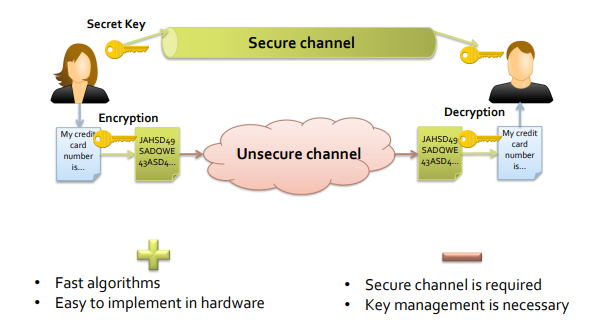
\includegraphics[width=.9\linewidth]{/home/eoshiru/library/docs/knowledge-database/static/images/sym-methods.png}
\end{center}
\item both participants use the same key (for de- and encryption)
\item the key therefore has to be transmitted aswell (risk)
\end{itemize}
\item two keys (asymmetric algorithms)
\begin{itemize}
\item \begin{center}
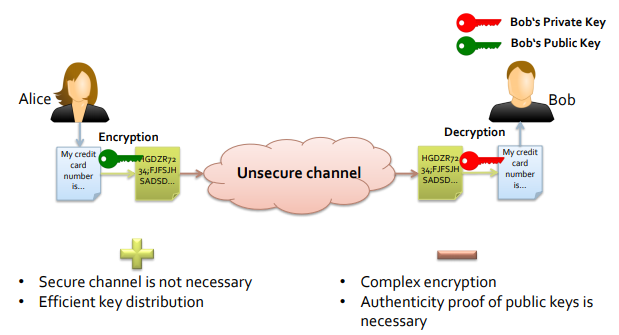
\includegraphics[width=.9\linewidth]{/home/eoshiru/library/docs/knowledge-database/static/images/asym-methods.png}
\end{center}
\item a public key is used to encrypt a message which can only be decrypted with the according private key \(\rightarrow\) private key is not submitted (thus more secure)
\end{itemize}
\item hybrid methods
\begin{itemize}
\item \begin{center}
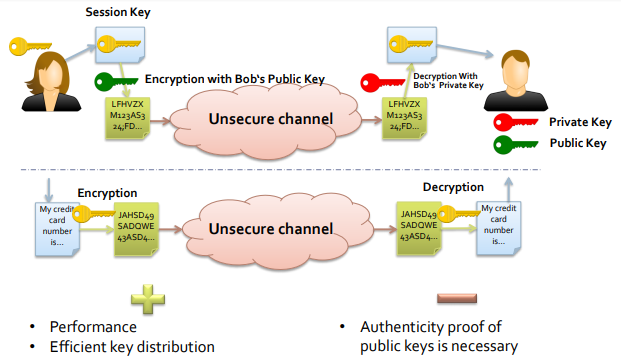
\includegraphics[width=.9\linewidth]{/home/eoshiru/library/docs/knowledge-database/static/images/hybrid-methods.png}
\end{center}
\item session key is encrypted with public key and transmitted and then gets decrypted with private key
\item session key is used to encrypt data/message and now the receiver can decrypt it with the earlier decrypted session key
\end{itemize}
\item one-way hash functions
\begin{itemize}
\item \textbf{compression}
\begin{itemize}
\item inputs of arbitrary length are mapped to outputs with fixed length
\end{itemize}
\item \textbf{irreversibility} (surjective function)
\begin{itemize}
\item input can not be inferred from the output
\end{itemize}
\item \textbf{collision-resistant}
\begin{itemize}
\item a hash function \(h()\) is called collision resistant - if it is hard to find to find two inputs \(a\) and \(b\) such that \(h(a)=h(b)\) and \(a \neq b\)
\end{itemize}
\end{itemize}
\end{itemize}

\href{https://www.youtube.com/watch?v=YEBfamv-\_do\&feature=youtu.be}{Public key cryptography visualized}

Challenge-Response with Public Key:
\begin{enumerate}
\item Client sends identifier ID to server
\item Server sends generated random number R
\item Client signs R with a private key \& sends the result
\item Server verifies the result using the public key of the client
\end{enumerate}
\subsection{Public Key Infrastructure (PKI)}
\label{sec:org6a37fa7}
\begin{itemize}
\item Challenge: management of public keys
\item binding the key to its owner
\begin{itemize}
\item certificate = digital certificate of public key assignment to a (legal) person (eg X.509 Certificate)
\item certification authority (CA) = provides certificate issugin services; the certificates are usually signed with the private key of the CA
\begin{itemize}
\item reduces the problem of authentic key distribution to distribution of authentic keys of CAs
\end{itemize}
\item service users must identify themselves to the CA
\end{itemize}
\end{itemize}

CA services require the use of a computer which is suitably protected against improper use. In particular, it is recommended to use a computer without any network connection to protect it physically.\\
The secret keys of the CA must be adequately protected and may not be given to third parties. The responsibility lies with the administrators of the CA, who are, therefore, advised to use external peripheral devices (eg smart card, floppy disk).\\
The secret signature key of the CA must only be used to sign CA- or Enduser keys or revocation lists (CRLs) or to create cross-signed certificates.\\
Each CA must generate its asymmetric key pairs by themselves. Asymmetric key pairs of the CA for signature generation must have a minimum length of 2048 bits RSA (or equivalent). In case CA generates asymmetric key pairs fo the end user, CA has to perform it on a dedicated CA computer.\\
All data obtained during certification must be treaded as confidential by the CA staff. CA legal data protection regulations are to be complied with.\\

In summary the operation of a Certificate Authority is mainly influenced by the \emph{technical requirements}, the \emph{legal requirements} and the \emph{organizational requirements}.
\section{SSL/TLS}
\label{sec:orgdce2239}
Wiki: Transport Layer Security (TLS), and its now-deprecated predecessor, Secure Sockets Layer (SSL), are cryptographic protocols designed to provide communications security over a computer network. Several versions of the protocols find widespread use in applications such as web browsing, email, instant messaging, and voice over IP (VoIP). Websites can use TLS to secure all communications between their servers and web browsers.

The TLS protocol aims primarily to provide privacy and data integrity between two or more communicating computer applications.[2]:3 When secured by TLS, connections between a client (e.g., a web browser) and a server (e.g., wikipedia.org) should have one or more of the following properties:
\begin{itemize}
\item The connection is private (or secure) because symmetric cryptography is used to encrypt the data transmitted. The keys for this symmetric encryption are generated uniquely for each connection and are based on a shared secret that was negotiated at the start of the session (see § TLS handshake). The server and client negotiate the details of which encryption algorithm and cryptographic keys to use before the first byte of data is transmitted (see § Algorithm below). The negotiation of a shared secret is both secure (the negotiated secret is unavailable to eavesdroppers and cannot be obtained, even by an attacker who places themselves in the middle of the connection) and reliable (no attacker can modify the communications during the negotiation without being detected).
\item The identity of the communicating parties can be authenticated using public-key cryptography. This authentication can be made optional, but is generally required for at least one of the parties (typically the server).
\item The connection is reliable because each message transmitted includes a message integrity check using a message authentication code to prevent undetected loss or alteration of the data during transmission.
\end{itemize}

In the OSI-model SSL/TLS belongs in layer 6, in the TCP/IP model it belongs above the transport layer (ie TCP,..) and below the application layer (ie HTTP,..).

The SSL/TLS Architecture basically consists of of 2 protocol layers:\\
\begin{center}
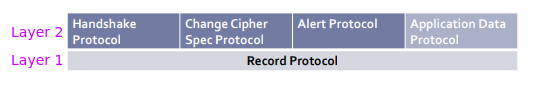
\includegraphics[width=.9\linewidth]{/home/eoshiru/library/docs/knowledge-database/static/images/ssl-layer.png}
\end{center}

\subsection{Record Protocol (Layer 1)}
\label{sec:orgf3abffb}
\begin{itemize}
\item represents the lower level of the TLS protocol
\item encapsulation of exchanged messages
\item decomposition into blocks for transmission
\item end-to-end encryption
\begin{itemize}
\item symmetric algorithms
\item see the following handshake protocol
\end{itemize}
\item integrity and authenticity are ensured by cryptographic checksums
\end{itemize}

\begin{center}
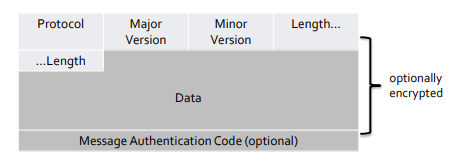
\includegraphics[width=.9\linewidth]{/home/eoshiru/library/docs/knowledge-database/static/images/record-protocol.png}
\end{center}

\subsection{Handshake Protocol (Layer 2)}
\label{sec:org04342a3}
\begin{itemize}
\item server and client decide on:
\begin{itemize}
\item mode of encryption
\item type of message authentication
\item secret key
\end{itemize}
\item authentication via certificates is possible
\end{itemize}

\begin{center}
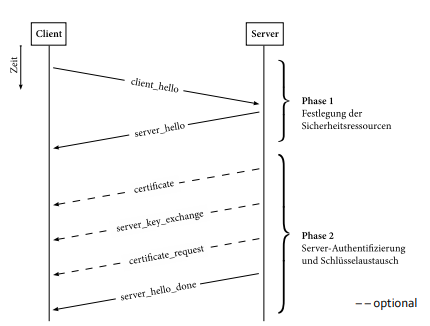
\includegraphics[width=.9\linewidth]{/home/eoshiru/library/docs/knowledge-database/static/images/handshake-protocol-1.png}
\end{center}
\begin{center}
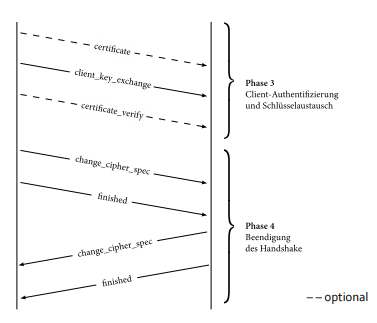
\includegraphics[width=.9\linewidth]{/home/eoshiru/library/docs/knowledge-database/static/images/handshake-protocol-2.png}
\end{center}

\subsection{Change Cipher Spec Protocol (Layer 2)}
\label{sec:org734de4d}
\begin{itemize}
\item change to the negotiated cipher suite
\item cipher suite identifies a combination of four algorithms
\begin{itemize}
\item key exchange
\item authentication
\item hash function
\item encryption
\end{itemize}
\end{itemize}

\subsection{Alert Protocol (Layer 2)}
\label{sec:org921007b}
\begin{itemize}
\item signaling on error states
\item protocol defines two fields:
\begin{itemize}
\item level of error alert
\begin{itemize}
\item warning
\item fatal \(\rightarrow\) connection is immediately interrupted
\end{itemize}
\item type of error alert
\begin{itemize}
\item detailed error description
\end{itemize}
\end{itemize}
\end{itemize}

\subsection{Application Data Protocol (Layer 2)}
\label{sec:org2f79164}
\begin{itemize}
\item pass application data transparently
\begin{itemize}
\item without consideration of its content
\end{itemize}
\item based on security parameters data is\ldots{}
\begin{itemize}
\item fragmented
\item compressed
\item protected
\item encrypted
\end{itemize}
\end{itemize}

\noindent\rule{\textwidth}{0.5pt}
\subsubsection{Further Reads}
\label{sec:orgda8aa1c}
\begin{itemize}
\item \url{https://www.cloudflare.com/learning/ddos/glossary/tcp-ip/}
\item \url{https://www.cloudflare.com/learning/ssl/what-happens-in-a-tls-handshake/}
\end{itemize}
\section{Authentication}
\label{sec:org5405c6e}
\subsection{Introduction}
\label{sec:org1abc15a}
Authentication is the process of verficating if someone is the one who he claims to be. There are different kinds of authenticators:
\begin{itemize}
\item knowledge-based
\begin{itemize}
\item PIN, passwords
\item Challenge-Response
\end{itemize}
\item biometrics
\begin{itemize}
\item fingerprint, iris, voice, signature, keystroke behavior
\end{itemize}
\item ownership-based
\begin{itemize}
\item something that you do not notice, but what is stored on a medium
\item IDs, magnetic cards, certificates, smart cards
\end{itemize}
\item multi-factor authentication
\begin{itemize}
\item combination of different types of authentication
\item 2 Factors: eg deposit card + PIN, credit card + signature, password + PIN sent by SMS
\item 3 Factors: eg password + smart card + fingerprint
\end{itemize}
\end{itemize}

\subsubsection{Knowledge-based Authentication}
\label{sec:org2b80c77}
Knowledge-based Authentication using passwords
\begin{itemize}
\item Alice agrees with Bob on a secret password p for authentication of Alice to Bob
\item Bob applies a one-way or cryptographic hash function H on the password, and stores the image value H(p)
\item when authenticating the password is send and then gets hashed again and compared to the stored hash
\end{itemize}

\subsection{Kerberos}
\label{sec:org0ac6e8b}
Wiki: Kerberos is a computer-network authentication protocol that works on the basis of tickets to allow nodes communicating over a non-secure network to prove their identity to one another in a secure manner.

\begin{itemize}
\item works according to the KDC principle
\item \emph{User} wants to use a certain service
\item \emph{Client} is the local Kerberos application
\item \emph{Server} provides the desired service
\item \emph{Authentication Server (AS)} is used for primary user authentication
\item Ticket Granting Server (TGS) issues tickets for certain services
\item KDC includes AS and TGS
\end{itemize}

\subsubsection{Accreditation}
\label{sec:orga10948f}
\begin{itemize}
\item User and his password are provided to the AS
\item TGS and its secret key are also accredited by the AS
\item Server and its secret key are made known to the TGS
\end{itemize}

See pages 5 - 12 for more on Kerberos

\section{Identity Information in Directory Services}
\label{sec:org480c9f8}
\begin{itemize}
\item directory service is a special 'name service'
\item property-based requests
\begin{itemize}
\item comparison: full-name DNS request
\item similar to 'Yellow Pages'
\end{itemize}
\item OSI X.500 is the 'classical' Directory Service
\begin{itemize}
\item however the complex 'Directory Access Protocol' (DAP) prevented it from becoming more widespread
\end{itemize}
\item LDAP = Lightweight Directory Access Protocol
\begin{itemize}
\item standardized by IETF
\end{itemize}
\end{itemize}

Important: See pages 14 - 23
\section{Management of Access Rights}
\label{sec:org22973b3}
\textbf{Authorization} is the process of verification and access right assignment for a resource/service to a subject and is not to be confused with \emph{Authentication} which is the process of verificating claimed properties. Access Control is a process of access rights management and control.

\textbf{Access Matrix}\\
\begin{center}
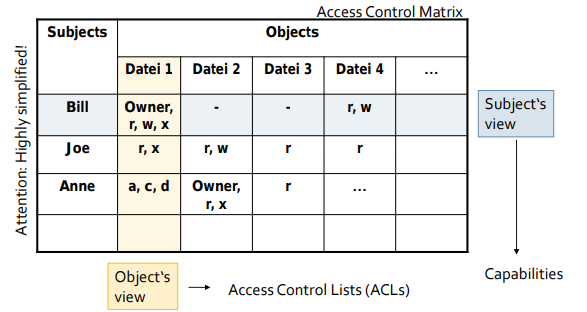
\includegraphics[width=.9\linewidth]{/home/eoshiru/library/docs/knowledge-database/static/images/access-matrix.png}
\end{center}
\begin{itemize}
\item group- and role-based access rights management:
\begin{itemize}
\item complexity reduction by clustering users into 'role groups'
\item inheritance relationships in rights management
\item permissions based on roles
\end{itemize}
\end{itemize}

\textbf{Access Control Lists}\\
\begin{center}
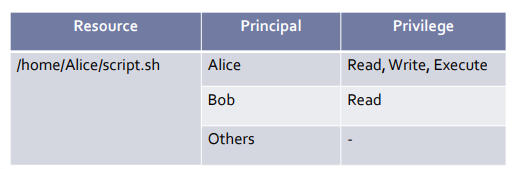
\includegraphics[width=.9\linewidth]{/home/eoshiru/library/docs/knowledge-database/static/images/access-list.png}
\end{center}
\begin{itemize}
\item \emph{principal} is a user, group or process that can be authenticated
\item simply put: ACL is a set/list of resources, principals and corresponding access rights
\end{itemize}

\textbf{Access Control Models}\\
\begin{itemize}
\item Discretionary Access Control (DAC)
\begin{itemize}
\item access rights are assigned per user
\item owner of a resource can pass his own rights
\end{itemize}
\item Mandatory Access Control (MAC)
\begin{itemize}
\item rights passing is not allowed
\item the system alone decides on which user has access to which resources
\end{itemize}
\item Role-Based Access Control (RBAC)
\begin{itemize}
\item user could potentially be assigned multiple roles
\item access rights are role-based
\end{itemize}
\end{itemize}

\subsection{Realization in Operating Systems}
\label{sec:org64cfdd6}

Unix/Linux
\begin{itemize}
\item data/directories are associated to an inode descriptor (contains ID of the owner, ID of the group, ACL etc)
\item assignment of rights to the file owner, group, everyone else
\end{itemize}

Windows 2000/XP/Vista/7
\begin{itemize}
\item permissions/restrictions can be assigned to individual users and groups
\item security descriptors contain owner-ID, group-ID, Access Control Elements with Allow/Deny entries, logging operations
\end{itemize}

\section{Internet Firewalls (Chapter 6)}
\label{sec:org628b9b4}
Definition: Firewalls are hard- or software components, which control the interconnection point between two network areas and implement security strategies by restricting packet forwarding.

Fundamentals:
\begin{itemize}
\item Packet filter
\begin{itemize}
\item entity, which selectively processes flowing packets according to predefined rules, in particular, preventing packet forwarding
\end{itemize}
\item Proxy approaches
\begin{itemize}
\item representative of a client process
\end{itemize}
\item Network Address Translation (NAT)
\begin{itemize}
\item address translation, public and private addresses are distinguished
\end{itemize}
\item Bastion Host
\begin{itemize}
\item computer with particularly high protection requirements; vulnerability mainly results from the computer's exposed location
\end{itemize}
\item Dual-Homed Host
\begin{itemize}
\item computer with at least two network interfaces for two different subnets
\end{itemize}
\end{itemize}

These approaches are now covered in more detail.
\subsection{Packet Filter}
\label{sec:orga1f8abd}
\begin{center}
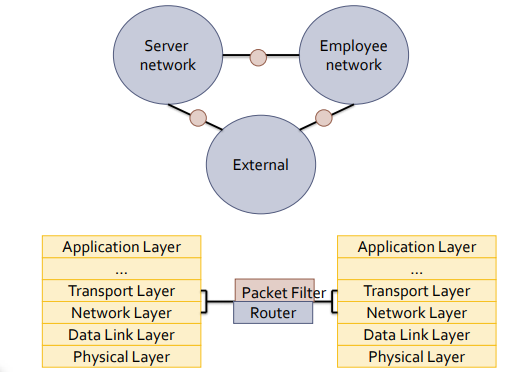
\includegraphics[width=.9\linewidth]{/home/eoshiru/library/docs/knowledge-database/static/images/packet-filter.png}
\end{center}

Then there are also router filter rules for example \texttt{deny icmp 129.12.0.0 0.0.255.255 any} in Linux environments this can be done via iptables, ipchains, ipfilter, \ldots{}\\
There are also dynamic packet filters:\\
\begin{center}
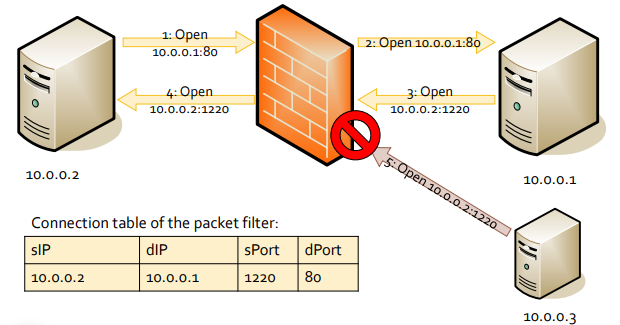
\includegraphics[width=.9\linewidth]{/home/eoshiru/library/docs/knowledge-database/static/images/dynamic-packet-filter.png}
\end{center}

Filter Table Guidelines
\begin{itemize}
\item "default deny" \(\rightarrow\) prohibit everything, which is not explicitly allowed
\item order \(\rightarrow\) filter table is usually processed sequentially, analysis is terminated after all the rules have been applied
\begin{itemize}
\item correct order should be maintained
\end{itemize}
\item prevent spoofing attacks
\begin{itemize}
\item packets coming from 'outside' with 'inside' addresses are rejected; the same holds true in the other direction if the source address is not an 'inside' address
\end{itemize}
\item static filters: UDP blocking
\item controlled handling of ICMP
\item prevent source-routing
\item efficiency: unneccessary filtering rules have to be removed
\end{itemize}

\subsection{Proxy Firewall}
\label{sec:orgab60ae5}
\begin{center}
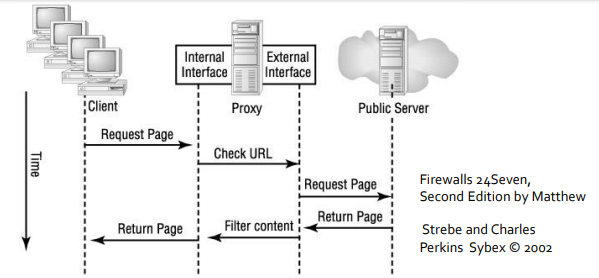
\includegraphics[width=.9\linewidth]{/home/eoshiru/library/docs/knowledge-database/static/images/proxy-firewall.png}
\end{center}
\begin{itemize}
\item typically at transport layer or as an application proxy
\item transport layer: requires client code modification
\item application proxy: can perform service-specific controls
\end{itemize}

\subsection{Network Address Translation}
\label{sec:org1a3fed5}
NAT is a proxy concept at the network layer. Initially it was intended as a measure to preserve the IPv4 address space while today it is used to conceal internal network structures.
\begin{itemize}
\item doing NAT in practice gives up the end-to-end principle as it leads to numerous diffuclties (eg ftp)
\end{itemize}

\begin{center}
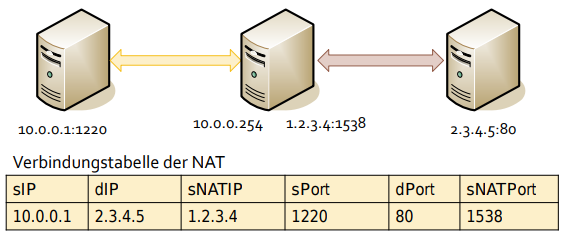
\includegraphics[width=.9\linewidth]{/home/eoshiru/library/docs/knowledge-database/static/images/NAT.png}
\end{center}

\subsection{Architectures}
\label{sec:org646f30e}
Let's look at different architectures utilizing different kinds of firewalls:\\
\begin{center}
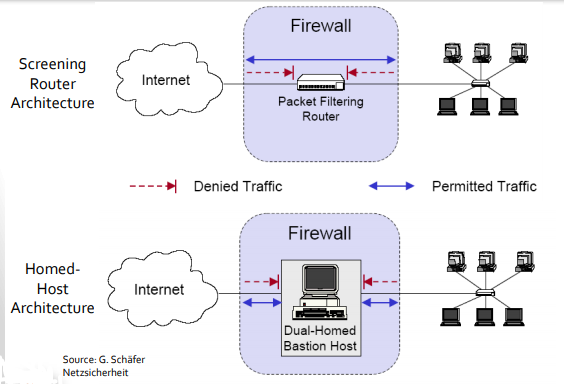
\includegraphics[width=.9\linewidth]{/home/eoshiru/library/docs/knowledge-database/static/images/architectures-1.png}
\end{center}
\begin{center}
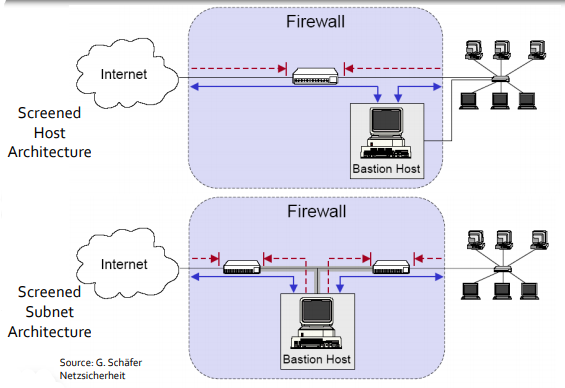
\includegraphics[width=.9\linewidth]{/home/eoshiru/library/docs/knowledge-database/static/images/architectures-2.png}
\end{center}
\begin{center}
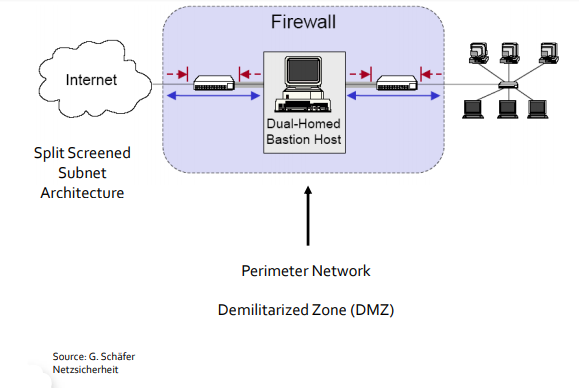
\includegraphics[width=.9\linewidth]{/home/eoshiru/library/docs/knowledge-database/static/images/architectures-3.png}
\end{center}

One traditional conception in network design has been that of the "perimeter" which means that there's an "inside" and "outside" to our network. However this is not applicable to the modern situation because of eg
\begin{itemize}
\item mobile devices
\item peer-to-peer systems
\item ubiquitous computing
\item ad-hoc networks
\item sensor networks
\item \ldots{}
\end{itemize}

So there is no clearly defined "perimeter network" available anymore.

\subsection{IT-Security Management Aspects}
\label{sec:orga35ccd0}
\begin{itemize}
\item determination of the required security level
\item firewall placement and coordination
\begin{itemize}
\item clear transition between 'internal' and 'external'?
\item select entrance architecture (dual homed, screened, subnet,..)
\item should the subnets be protected from one another?
\item do devices require 'personal firewalls'?
\item how can the three stages (entrace, subnet, end-system) be kept consistent and checked for errors?
\end{itemize}
\item Analysis of open communication channels
\begin{itemize}
\item dependencies on the first point
\item administration concept: who gets to issue which rules?
\end{itemize}
\item firewall management requires security policy support
\end{itemize}

\section{Intrusion Detection Systems (Chapter 7)}
\label{sec:org34d5c4f}
Motivation:
\begin{itemize}
\item computer has been compromized and is used for (illegal) data distribution
\item network operator performs IP accounting and finds out that a computer, which has previously generated next to no load, is suddenly generating a high amount of it
\item Goal: attack detection and intrusion detection alarm
\end{itemize}

Intrusion Detection Systems
\begin{itemize}
\item find and report suspicious activity in systems and networks
\item intrusion prevention: initiation of control measures
\begin{itemize}
\item intrusion response
\end{itemize}
\end{itemize}

\subsection{Classification of Intrusion Detection Systems}
\label{sec:org19909ed}
Location:
\begin{itemize}
\item Host-based
\begin{itemize}
\item system breach and misuse detection
\item examination of log files
\item integrity checks by checksums
\item inspection of "privilege escalation"
\end{itemize}
\item Network-based
\begin{itemize}
\item monitoring and verification of network traffic, which can take place at various network locations
\end{itemize}
\item Hybrid
\end{itemize}

Detection:
\begin{itemize}
\item signature-based
\item anomaly-based
\end{itemize}

\subsubsection{Signature-based Detection}
\label{sec:org1443489}
\begin{itemize}
\item break-in (attempt) detection based on known procedures
\begin{itemize}
\item eg buffer overflow attack
\item eg implies \emph{default.ida} within a URL in an HTTP packet together with a certain pattern in the URL Argument Name Field is a Code Red attack
\end{itemize}
\item signatures must (same holds true for virus scanners) be kept up-to-date
\item challenges:
\begin{itemize}
\item register the attacks
\item describe the attacks
\item errors of type 1 and 2 (classification problem)
\end{itemize}
\end{itemize}

\subsubsection{Anomaly-based Detection}
\label{sec:org3bffd78}
\begin{itemize}
\item detection of "normal" user behaviour deviations
\item normal behaviour has to be statically describable
\item classification problem
\item normal behaviour should be determined through learning
\item very effective attacks which are not deviating much from normal user behaviour might remain undetected
\end{itemize}

\begin{enumerate}
\item Example: Securing Gateways
\label{sec:orgb3340b6}
\begin{center}
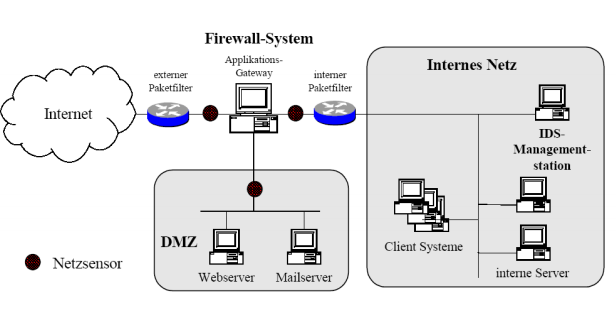
\includegraphics[width=.9\linewidth]{/home/eoshiru/library/docs/knowledge-database/static/images/gateways.png}
\end{center}
\end{enumerate}

\subsection{Intrusion Detection System - Honeypots}
\label{sec:org96a3823}
Approach:
\begin{itemize}
\item place unsecured server/service ("honeypot") in the network
\item monitor honeypots
\item analyse attacks and compromises
\begin{itemize}
\item identify tools, tactics and intruder motives
\end{itemize}
\end{itemize}

Typical objectives:
\begin{itemize}
\item detect botnet attacks
\begin{itemize}
\item botnet = network of compromized computers that can be remotely orchestrated by the attacker
\end{itemize}
\item detect phishing attacks
\end{itemize}

\subsection{IDS in IT-Security Management}
\label{sec:org79dd814}
\begin{itemize}
\item Intrusion Detection is a reactive IT-security approach
\begin{itemize}
\item complements preventive measures, such as firewalls
\end{itemize}
\item data protection legal requirements must be met
\item intrusion prevention (response): given automatic reactions, one has to make sure they cannot be used as an attack themselves (such as Denial of Service)
\item integration with network management is appropriate and necessary
\end{itemize}

\section{Incident Management (Chapter 8)}
\label{sec:org04273d5}
\subsection{History of CERTs / CSIRTs}
\label{sec:org1224f4a}
\begin{itemize}
\item CERT = Computer Emergency Response Team
\item CIRT = Computer Security Indicent Response Team

\item trigger: internet worm 1988
\item need of an IT-security 'fire brigage' became evident
\item CERT/CC (Coordination Center) was founded by DARPA located at CMU
\end{itemize}

Today:
\begin{itemize}
\item not just 'response', but generally incident handling
\item many CERTs and CSIRTs in the world eg DFN-CERT, CERT-Bund
\item in Germany: CERT-network
\item international network: FIRST (Forum of Incident Response and Security Teams)
\end{itemize}

\subsection{CSIRTs Tasks}
\label{sec:orgba47e2a}
Reactive Services
\begin{itemize}
\item alerts and warnings
\item incident handling
\begin{itemize}
\item incident analysis
\item incident response on site
\item incident response support
\item incident response coordination
\end{itemize}
\item vulnerability handling
\begin{itemize}
\item vulnerability analysis
\item vulnerability response
\item vulnerability response coordination
\end{itemize}
\item artifact handling
\begin{itemize}
\item artifact analysis
\item artifact response
\item artifact response coordination
\end{itemize}
\end{itemize}

Proactive Services
\begin{itemize}
\item announcements
\item technology watch
\item security audit or assessments
\item configuration \& maintenance of security tools, applications \& infrastructures
\item development of security tools
\item intrusion detection services
\item security related information dissemination
\end{itemize}

Security Quality Management Services
\begin{itemize}
\item risk analysis
\item business continuity \& disaster recovery planning
\item security consulting
\item awareness building
\item education/training
\item product evaluation or certification
\end{itemize}

\begin{enumerate}
\item Incident Handling
\label{sec:orgb547303}
\begin{center}
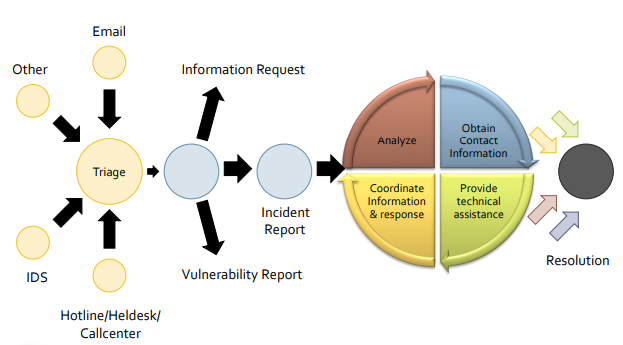
\includegraphics[width=.9\linewidth]{/home/eoshiru/library/docs/knowledge-database/static/images/incident-handling.png}
\end{center}

\item Coordination: Early Warning System
\label{sec:org8f5fcd0}
\begin{center}
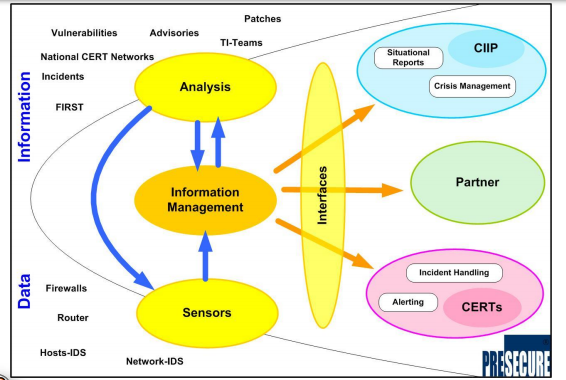
\includegraphics[width=.9\linewidth]{/home/eoshiru/library/docs/knowledge-database/static/images/early-warning.png}
\end{center}
\end{enumerate}

\subsubsection{Naming of Vulnerabilities}
\label{sec:org26fb7a7}
Naming requires standardization
\begin{itemize}
\item otherwise cooperation \& coordination become complex
\end{itemize}

Standard: common vulnerabilities and exposures
\begin{itemize}
\item managed by The Mitre Corporation
\end{itemize}

Example:

Name: CVE-2004-0309\\
Description: Stack-based buffer overflow in the SMTP service support in vsmon.exe in Zone Labs ZoneAlarm before 4.5.538.001, ZoneLabs Integrity client 4.0 before 4.0.146.046, and 4.5 before 4.5.085, allows remote attackers to execute arbitrary code via a long RCPT TO argument.\\
Status: Entry\\
Reference: BUGTRAQ:20040219 EEYE: ZoneLabs SMTP Processing Buffer Overflow\\
Reference: CERT-VN:VU\#619982 

\textbf{Part III: Trustworthy Software Engineering}\\

Trustworthy Software
\begin{itemize}
\item in Cordis.Europa.Eu security document defined as: Trustworthiness can be seen as software and infrastructure that is secure, reliable and resilient to attacks and operational failures; guaranteeing quality of service; protecting user data; ensuring privacy and providing usable and trusted tools to support the user in his/her security management.
\item trustworthiness needs to be considered from the outset rather than being addressed as add-on feature
\end{itemize}

So we focus on: Identity \& Security By Design (SBD)
\begin{itemize}
\item who is it for?
\item why does it matter?
\item what is it all about?
\item where does it apply?
\item when to apply?
\item how to apply?
\end{itemize}

\section{Identity (Chapter 1)}
\label{sec:org1887131}
Internet as a danger zone in terms of identity
\begin{itemize}
\item what exactly needs to be protected?
\item what should one orient towards?
\item which data is exceptionally worthy of protection?
\end{itemize}

Security vs Identity
\begin{itemize}
\item for starters: keynote by Dick Hardt at WWW 2007 on "Identity 2.0"
\item speech on identity by Kim Cameron
\end{itemize}

\subsection{Identity - Problem}
\label{sec:org80f20c6}
\begin{itemize}
\item Kim Cameron: "The internet was built without a way to know who and what you are connecting to."
\item initial situation:
\begin{itemize}
\item internet services are left on their own
\begin{itemize}
\item must provide security \(\rightarrow\) isolated identity solutions
\end{itemize}
\item criminalization of internet
\begin{itemize}
\item leads to loss of internet's credibility, for example drawback for e-businesses
\end{itemize}
\item identity layers are complex
\begin{itemize}
\item successful attemps, such as SSL and Kerberos - however overall too many different scenarios are required, so agreement is difficult
\end{itemize}
\end{itemize}
\end{itemize}

Possible solution: Identity Metasystem
\begin{itemize}
\item such a system provides confidential support to ensure who is connecting to whom/what on the internet
\item many questions:
\begin{itemize}
\item who holds the data?
\item who trusts whom?
\item what scales?
\item how does one realize openness to new developments that do not yet exist?
\end{itemize}
\end{itemize}

\subsection{Identity - Identity in Detail}
\label{sec:org68be60f}
\begin{itemize}
\item there are numerous definitions of identity, the lecture is based on Kim Cameron's definition: "\emph{Digital identity is a set of \textbf{claims}, which are made by a \textbf{digital subject} about self or other subjects.}"
\begin{itemize}
\item digital subject = person or thing (referred or real) in a digital realm that is described or with which one is dealing
\begin{itemize}
\item "with which one is dealing" = often in the context with request/response model
\item example digital subject: real persons, devices, resources, rules/policies and relationships between digitial subjects
\item discussions of the 'subject' term extend into philosophy
\end{itemize}
\item claim = claim suggests that something is true, typically something that seems to be controversial or questionable
\begin{itemize}
\item remark: claim is a relationship between a certain instance, a digital subject and an identity attribute
\end{itemize}
\end{itemize}
\end{itemize}

We must be able to \textbf{structure our understanding} of digital identity:
\begin{itemize}
\item we need a way to avoid returning to the \textbf{Empty Page} every time we talk about digital identity
\item we need to inform peoples' thinking by teasing apart the factors and dynamics explaining the successes and failures of identity systems since the 1970s
\item we need to develop hypotheses - resulting from observation - that are testable and can be disproved
\item our goals must be pragmatic, bounding our inquiry, with the aim of defining the characteristics of an unifying identity metasystem
\item the "\textbf{Laws of Identity}" offer a good way to express this thought
\item beyond mere conversation, the Blogosphere offers us \textbf{a crucible}
\begin{itemize}
\item the concept has been to employ this crucible to \emph{harden and deepen the laws}
\end{itemize}
\end{itemize}

These definitions embrace Kerberos, X.509, SAML. They take this problem of the evaluation of the usefulness of a digital identity up to a higher level in the systems sense of multiple layers. These definitions separate the layer of where stuff is communicated from the layer where evaluations are done – a very important step forward.

\subsection{Identity - Laws of Identity}
\label{sec:orgd080492}
\begin{enumerate}
\item \textbf{User Control and Consent}
\begin{itemize}
\item \emph{digital identity systems must only reveal information identifying a user with the user's consent}
\begin{itemize}
\item systems need to appeal in their convenience \& simplicity
\item constantly care about users' confidence
\begin{itemize}
\item requires holistic commitment
\item user must be cetral to control with respect to which identities are used and which data is made public
\item system must protect from deception (eg website location and missue)
\item system must inform the user of possible consequences upon certain action (data sharing, login etc)
\item the holistic approach must be used as a paradigm in all contexts (eg when logging into a company or a private blog it should always be clear that the user consents to the release of certain)
\end{itemize}
\end{itemize}
\end{itemize}
\item \textbf{Minimal Disclosure for a Constrained Use}
\begin{itemize}
\item \emph{the solution that discloses the least identifying information and best limits its use is the most stable long term solution}
\begin{itemize}
\item one should assume that data/information violations are unavoidable
\item to reduce risks, information use should be checked with respect to 2 strategies: "must be obtained" or "must be saved"
\item less information implies less value implies less risk
\item "as little as possible identification information" means:
\begin{itemize}
\item reduction of linkable information
\item use of claim transformations
\end{itemize}
\item avoid unnecessary information storage for "possible future" use (why should a credit card be stored by the shop?)
\item the law is closely related to information disasters
\end{itemize}
\end{itemize}
\item \textbf{Justifiable Parties}
\begin{itemize}
\item \emph{Digital identity systems must limit disclosure of identifying information to parties having a necessary and justifiable place in a given identity relationship}
\begin{itemize}
\item user has to have a clear understanding of whom the information is/will be exchanged with
\item system itself may not draw conclusions about relationships between subject and parties (eg Microsoft Passport is useful for logging into MSN but why should it know if I login to Google or eBay?)
\item in which situations are regulatory identities required?
\item same holds for intermediaries (what should they know to achieve their goal)
\item all participants must submit statements of how the information will be used
\end{itemize}
\end{itemize}
\item \textbf{Directed Identity}
\begin{itemize}
\item /a unifying identity metasystem must support both "omni-directional" identifiers for public entities and "unidirectional" identifiers for private entities
\begin{itemize}
\item digital identity should always be viewed in the context of another identity or a set of identities
\item omni-directional = public entities require "beacons" (publicly known identifier or URI) \(\rightarrow\) eg websites (URLs) or public devices
\item uni-directional = private entities (people) require an ability not to be turned into a beacon
\begin{itemize}
\item they require a unidirectional identifier, which can be used in combination with a trusted beacon (no correlation, eg user-bank interaction)
\item negative examples: bluetooth and RFID, partially WLAN
\end{itemize}
\end{itemize}
\end{itemize}
\item \textbf{Pluralism of Operators and Technologies}
\begin{itemize}
\item \emph{a unifying identity metasystem must channel and enable the inter-working of multiple identity technologies run by multiple identity providers}
\begin{itemize}
\item system may be ideal with respect to one characteristic, but not with respect to another
\item example: Authority vs Employer vs Individual
\item old and new technologies must be used and co-exist; identity system must not be in competition with technology, but must use it
\item technologies may have more growth than others (identity ecology)
\end{itemize}
\end{itemize}
\item \textbf{Human Integration}
\begin{itemize}
\item \emph{a unifying identity metasystem must define the human user as a component integrated through protected and unambiguous human-machine communications}
\begin{itemize}
\item communication can be completely secure but what about the last two meters (off the screen and into the eyes of the viewer); does the user really know who it is he's communicating with?
\begin{itemize}
\item phishing attacks are a good example of this
\end{itemize}
\item protocol for use of safety issues has to become a ceremony, absolutely predictable and controlled
\begin{itemize}
\item example: communication in the cockpit (channel 9 on United Airlines)
\end{itemize}
\end{itemize}
\end{itemize}
\item \textbf{Consistent Experience Across Contexts}
\begin{itemize}
\item \emph{a unifying identity metasystem must provide a simple consistent experience while enabling separation of contexts through multiple operators and technologies}
\begin{itemize}
\item simplicity and clarity are the main goal - identities have to be used in a similar fashion to all other things on the desktop
\begin{itemize}
\item user must be able to see, verify, add and remove identities
\end{itemize}
\item which type of identity is acceptable in which context?
\begin{itemize}
\item properties of such candidates are defined by the using parties
\item users must be able to recover the identity in the given context and understand which information is associated with it
\item person (human/legal) could possibly accept different types of identities
\item user must be able to choose the best identity in his opinion
\end{itemize}
\end{itemize}
\end{itemize}
\end{enumerate}
\textbf{Part III: Trustworthy Software Engineering}\\

\section{Identity in the Light of Privacy, Security and Trust (Chapter 2)}
\label{sec:orgd822daf}
\begin{itemize}
\item 7 Laws of Identity define requirements of dealing with identities
\begin{itemize}
\item first focus on conceptual/basic understanding
\end{itemize}
\item identity in global context has to comply with different levels
\begin{itemize}
\item layered approach of identity management:
\item \begin{center}
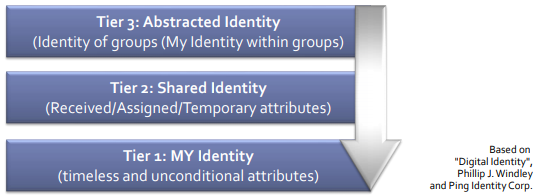
\includegraphics[width=.9\linewidth]{/home/eoshiru/library/docs/knowledge-database/static/images/identity-layers.png}
\end{center}
\end{itemize}
\end{itemize}
\subsection{Identity - Security - Privacy}
\label{sec:org179f50b}
\begin{itemize}
\item identity (in a digital setting) is often "only" closely linked to security, identity is more!
\begin{itemize}
\item security = protect data from unauthorized access, removal, tampering
\item privacy = protect attributes, preferences, etc which are associated with identity, against unnecessary use by subject
\item identity is in relation to others \(\rightarrow\) attributes realize trust relation ships
\end{itemize}
\end{itemize}
\subsection{Identity \& Trust}
\label{sec:orge9f2b39}
\begin{itemize}
\item Trust (wiki) = In a social context, trust has several connotations. Definitions of trust typically refer to a situation characterised by the following aspects: One party (trustor) is willing to rely on the actions of another party (trustee); the situation is directed to the future. In addition, the trustor (voluntarily or forcedly) abandons control over the actions performed by the trustee. As a consequence, the trustor is uncertain about the outcome of the other's actions; he can only develop and evaluate expectations. The uncertainty involves the risk of failure or harm to the trustor if the trustee will not behave as desired
\item \textbf{Trust = Conviction and belief in the sincerity, honesty and good intentions of another party with respect to a risk-prone action.}
\end{itemize}
\subsubsection{Trust examples}
\label{sec:org4425c64}
\begin{itemize}
\item shopping with credit card, which trust relationships \& risks exist?
\begin{itemize}
\item identity and Credit Card company
\item identity and service
\item identity/service and card register
\item identity/service and money
\end{itemize}
\item \(\rightarrow\) trust is always associated with risk
\item trust is something one connects to a person
\begin{itemize}
\item one cannot enforce trust by another person
\end{itemize}
\end{itemize}
\subsubsection{Trust properties}
\label{sec:orgbedf44f}
\begin{itemize}
\item trust is rarely transitive
\begin{itemize}
\item example: I trust Sara's taste in music, she, in turn, trusts Peter's - therefore I would possibly trust Peter in selecting music for my Birthday Party
\end{itemize}
\item trust cannot be shared
\begin{itemize}
\item example: A trusts B and C, which does not imply that B and C trust each other
\end{itemize}
\item trust is not symmetric
\begin{itemize}
\item example: if I trust you, you don't necessarily trust me in return
\end{itemize}
\item trustworthiness cannot be self-declared ("trust me!")
\item trust is a value closely related to evidence
\begin{itemize}
\item buying a brand computer which is more expensive because I trust the brand
\item Computer allows access upon login, since the provided evidence (login/password) serve as proof
\end{itemize}
\item trust is hard to quantify
\begin{itemize}
\item I trust Sara more than Peter - what does that mean?
\item in business context trust can be evaluated against risks (given obvious risk levels)
\item otherwise a contract is used as a basis: analysis is required, risks are evaluated and thereby cotractual relationships are defined; leads to Service Level Agreements (SLA) providers and users
\end{itemize}
\item Trust by reputation
\begin{itemize}
\item trust in a person can develop from other people's statements about him/her (Communities of Trust)
\item examples:
\begin{itemize}
\item all security experts advise caution when traveling in the following countries
\item ebay: one buys a product from a handler he doesnt know, but which has good reviews (high reputation)
\end{itemize}
\end{itemize}
\end{itemize}
\subsection{Identity \& Privacy}
\label{sec:org8d6704c}
\begin{itemize}
\item privacy is an important and complicated topic (tightly coupled with data protection)
\item identity and privacy are closely related
\begin{itemize}
\item what does privacy mean for a person?
\begin{itemize}
\item generally: private data shouldn't become public
\item however, often: private data disclosure is ok if it yields considerable benefits
\end{itemize}
\item privcacy must be observed in context
\begin{itemize}
\item eg discount systems: provide us your address and date of birth and we'll give you a 15\% discount
\end{itemize}
\end{itemize}
\item privacy is partially legally regulated
\begin{itemize}
\item eg Federal Data Protection Act, European Data Protection Directive, Patriot Act
\end{itemize}
\item conclusion in legal context: own applications systems must take identity and privacy into account (see Laws of Identity)
\begin{itemize}
\item embed the concepts of identity and privacy in design
\item use of identity and privacy-relevant information must be comprehensible, verifiable and reportable at any point in time
\item identity management system or an identity metasystem must be able to answer questions on identity privacy terms
\item legal requirements forcte system operators to testify on privacy policy
\begin{itemize}
\item eg webshop sends cookies to customers, what should the privacy policy say? (eg We use cookies)
\end{itemize}
\end{itemize}
\item privacy principle - respect privacy
\begin{itemize}
\item accountability
\item identifying purposes
\item requirement of affected person's consent
\item minimal privacy data collection (time limit)
\item limitations of use
\item data collection accuracy
\item protection
\item access to personal data (to the owner)
\item comprehensible regulations
\end{itemize}
\end{itemize}

\section{Identity Management Systems (Chapter 3)}
\label{sec:orge42d64e}
\begin{itemize}
\item what is needed for identity implemenation?
\begin{itemize}
\item some kind of \textbf{identity metasystem} \(\rightarrow\) contains 3 certain roles (can be more)
\item \textbf{identity provider}
\begin{itemize}
\item person or an organization, which creates digital identities, either for themselves or on behalf, eg online shop could create identities for customers, authorities provide identities for their employees
\end{itemize}
\item \textbf{relying party} (human/legal person)
\begin{itemize}
\item person or organization, which requires digital identity before allowing entry/acess
\item example: users willing to revoke a contract - the relying party defines which claims are required in order to execute cancellation, as well as which formats and credentials are accepted
\end{itemize}
\item \textbf{digital subject}
\begin{itemize}
\item individual or entity for which claims are made
\end{itemize}
\end{itemize}
\end{itemize}

Definition \textbf{Identity Management}: "Identity management is the set of processes, tools and social contracts surrounding the creation, maintenance and termination of a digital Identity for people or, more generally, for systems and services to enable secure access to an expanding set of systems and applications."

\textbf{Identity Management Lifecycle}\\
\begin{center}
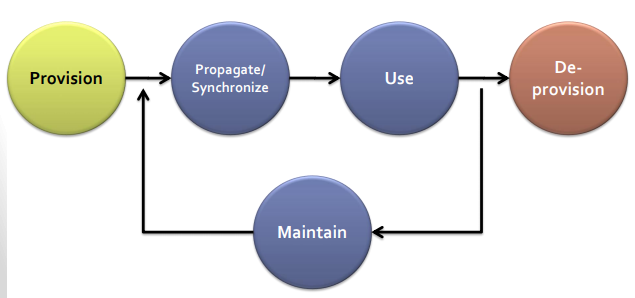
\includegraphics[width=.9\linewidth]{/home/eoshiru/library/docs/knowledge-database/static/images/identity-management-lifecycle.png}
\end{center}

There are three identity management levels:
\begin{itemize}
\item personal identity management
\item organization-related identity management
\item federated identity mangament
\end{itemize}

\subsubsection{Personal Identity Management}
\label{sec:orgd4b09e5}
Entity-perspective
\begin{itemize}
\item Management of different identities (different accounts for different systems)
\item Management and control of which information is provided to a service (z.B. Email, phone number etc.)
\item eg MS Passport, MS Cardspace
\end{itemize}
\subsubsection{Organization-related Identity Management}
\label{sec:org71ecda7}
Organizational perspective
\begin{itemize}
\item Management of identities of an organization
\item Different services of an organization are provided with and updated by identity information.
\item Traceability of data flows and data accesses
\item Management of privileges and roles within the organization
\item Definition of organization‘s policies as to the entities i.e. which data can be accessed
\item eg SUN Identity Management Suite (SUN Identity Manager), Microsoft Identity Integration Server, IBM Tivoli Identity Manager
\end{itemize}

\subsubsection{Federated identity Management}
\label{sec:org263110a}
What is meant by “Federation“?
\begin{itemize}
\item “Federation is an association of independent organizational units, which have
\end{itemize}
a trust relationship.“
\begin{itemize}
\item Among the latest developements in the field of IdM.
\item Is driven both by the state and industry
\begin{itemize}
\item Common and simplified resource access
\item Complex problems/business processes and a high level of specialization require cooperation.
\item Harmonization of business pocesses
\item Cost savings with respect to administration and resource use
\end{itemize}
\item Frequently used technologies
\begin{itemize}
\item SAML (Security Assertion Markup Language)
\item XML (Schema, Encryption, Signature etc.)
\item Web Service interfaces
\end{itemize}
\item Federation perspective
\begin{itemize}
\item association of organizational units, organizations or even nations
\item Shared use of resources and services of Federation partners
\item Cross-organizational business processes within the Federation
\item Modeling and definition of trust relationships
\item Federative services are then made available according to the defined trust relationships providing ease of access to resources/data (i.e. Single Sign-on)
\end{itemize}
\item Example projects/products/approaches: Liberty Alliance Projekt (SAML 2.0) , WS-Federation specification , SUN Identity Management Suite (SUN Federation/Access Manager) , Ping-ID, PingFederate , Shibboleth , FOAF+SSL
\end{itemize}

\subsection{Anticipitated Benefits of IDMS}
\label{sec:org757ba79}
Reduced management overhead
\begin{itemize}
\item Better optimization/automatization of business processes
\item Reduced time required for providing a new employee with access rights to resources
\item Reduced risk of a former employee accessing resources
\item Policy and legal requirement compliance support (privacy)
\item Data consistency (data matching, modification checks, …)
\item Standard interfaces (APIs, standards …) to data/services/resources
\end{itemize}

\subsection{Components of IDM systems}
\label{sec:orgf6a8fc6}
"he focus of identity management is on user provisioning — the creation, maintenance, and termination of user accounts and management of credentials in support of authentication and access control." (HurwitzGroup, 2001)\\
\begin{center}
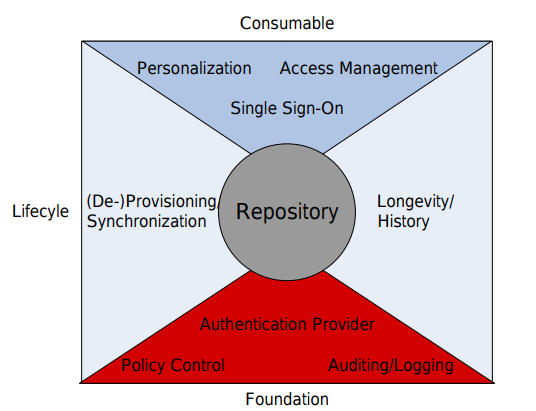
\includegraphics[width=.9\linewidth]{/home/eoshiru/library/docs/knowledge-database/static/images/idm-components.png}
\end{center}
\subsubsection{Basic Components}
\label{sec:org8d35c92}
\begin{itemize}
\item \textbf{Repository}
\begin{itemize}
\item Repository represents the core component for many identity management systems
\item It is a \textbf{logical data storage} (i.e. database, directory service), in which identity information, guidelines and other organization information can be stored
\end{itemize}
\item \textbf{Propagation}
\begin{itemize}
\item Depending on the system in use, an identity entry could need to be transferred from the current reposiroty to another one
\end{itemize}
\item \textbf{Authentication Provider/Identity Provider}
\begin{itemize}
\item is responsible for primary identity authentication
\item often issues a credential, which can be used for further authentication and authorization (z.B. SAML Token)
\item provides multiple interfaces (z.B. LDAP, Kerberos), by means of which service can perform authentication
\end{itemize}
\item \textbf{Policy Control}
\begin{itemize}
\item policy control governs rules of information usage, disclosure and logging
\item authorization policies determine which identity can access and manipualte which information
\item policy control monitors the defined guidelines, creates events to be audited and signalled of according to certain rules (for example, security warnings)
\end{itemize}
\item \textbf{Auditing, Monitoring}
\begin{itemize}
\item auditing provides necessary mechanisms for information detection and storage
\item that information normally contains access protocols and data operations (specifically in the repository)
\item if form a basis for tracking whether the policies are being adhered to and is used for subsequent security checks
\end{itemize}
\end{itemize}
\subsubsection{Lifecycle Components}
\label{sec:orgbf45ae2}
\begin{itemize}
\item \textbf{(De-)Provisioning and propagation/synchronization}
\begin{itemize}
\item applies automation of all the procedures and tools to manage the identity lifecycle
\item this Lifecycle is split into initial provosioning, synchronization and de-provisioning phases
\item in the initial provisioning phase the according service is supplied with the necessary identity information such that the new identity can use the service (provisioning process)
\item in the synchronzsation phase identity information is updated and compared between services (synchronization and propagation process)
\item in the de-provisioning phase all the identity information is removed (de-provisioning process)
\end{itemize}
\item \textbf{History, Longevity}
\begin{itemize}
\item History and longevity tools create historical records, by means of which one can examine evolution of an identity overtime (i.e. creation, activation, locking, new status, removal)
\item these components provide means for such activites as investigating whether or not a certain identity exists in the system and which changes it underwent
\end{itemize}
\end{itemize}
\subsubsection{Usage Components}
\label{sec:org4c02d04}
\begin{itemize}
\item \textbf{Single Sign-on}
\begin{itemize}
\item Single Sign-on enables an identity to perform its initial authentication and access numerous services and data without further re-authentication.
\item Initial authentication is typically performed by an associated Identity Provider, which issues a credential.
\item That Credential is then used to authenticate to other systems.
\end{itemize}
\item \textbf{Personalization}
\begin{itemize}
\item Personalization and preference management tools provide the identity an ability to set up individual settings for applications/services bound to that identity.
\end{itemize}
\item \textbf{Access Management}
\begin{itemize}
\item Similar to policy control
\item Identity can define policies as to which identity can access/modify which information.
\end{itemize}
\end{itemize}
\section{WAM (WebComposotion Architecture Model)}
\label{sec:orgda763ad}
WAM is a modeling language for designing distributed, organization-spanning web applications and (who would've thought) was developed by the lecturer/prof and is absolutely industry irrelevant for that matter. But hey that's just how things are at Chemnitz University. By the way are you looking for irrelevant + outdated material? You'd love to study some unstructured slides enhanced by Internet Explorer 6 screenshots? You hate effective use of slides and think that using results of pedagogical research to help students learn better is for nonbelievers? MAN I HAVE SOMETHING FOR YOU! Go to \url{https://www.tu-chemnitz.de} and get yourself the new and updated "Bullshit University Education"-StarterPack right now!
\end{document}
